

% Section: EVALUATION
\subsubsection{Experiment Setup}
\label{sec:prototype-evaluation}

We deploy the prototype of the regulation component of the cloud coordinator from community cloud management system
in the Community-Lab testbed, which is developed by the CONFINE European project~\cite{Braem2013}. 
The cloud coordinator components are installed on nodes of the Community-Lab testbed, 
which consist of Jetway JBC372F36W devices, and are equipped with an Intel Atom N2600 CPU, 4GB of RAM and 120GB SSD. % http://www.jetwaycomputer.com/JBC372F36.html
Depending on the experiment, one or two nodes operate as SNs, while each ON hosts between one and four VM instances. 
Note, however, that since OpenWRT has limited supported for either containers-based or full virtualization, 
in these experiments the nodes submit and process the requests but VMs are not actually created on the ONs.
The objectives of the experiments are twofold: 

\begin{enumerate}
    \item Experiment 1: Assess the prototype operation regarding the incentive-based resource assignment algorithm in a local community cloud scenario.
    \item Experiment 2: Study the coordination between SNs from different zones in the federated community cloud scenario with heterogeneous resource distribution.
\end{enumerate}


%%%%%%%%%%%%%%%%%%%%%%%%%%%%%%%%%%%%%%%%
%%%%%%%%%%%%%%%%%%%%%%%%%%%%%%%%%%%%%%%%
\subsubsection{Resource Assignment in Local Community Cloud Scenario}
\label{sec:resource-assign-local}

In order to study the performance of the prototype in a real deployment of a local community cloud, 
we install our software components in four ONs and one SN in Community-Lab testbed, 
which are connected to the Guifi.net community network. 
Each node behaves as an ON but with different configuration, in order to have a heterogeneous set of cloud resources. 
The four nodes include
f101 sharing 1 out of total 2 VMs, 
f102 sharing 3 out of total 3 VMs, 
f103 sharing 1 out of total 3 VMs, and
f104 sharing 1 out of total 1 VM.
Each ON sends request for VM instances to the SN at regular intervals. 
VMs are requested for 20 seconds interval at a time. 
Each ON requests as many VMs as its total capacity, for example node f101 always requests 2 VMs.
If the request is accepted by the SN, the ON obtains the VMs for the next 20 seconds. 
If the request is rejected, the ON waits for 5 seconds before making any further requests.
The experiment is run with this setup for around 5 minutes. 
We analyse the different aspects of the system behaviour in the following.


%%%%%%%%%%%%%%%%%%%%%%%%%%%%%%%%%%%%%%%%
\subsubsection{Resource Utilisation}

Figure~\ref{fig:resource-util-graphs} shows the level of resource utilisation in the system in terms of the number of reserved VMs versus the total number of VMs.
It can be seen that resource utilisation varies widely and 100\% utilisation, meaning all the VMs being occupied, occurs only for short intervals.
This is because as nodes obtain VMs they spend their credit, 
and if they are not able to earn credit by contributing VMs, 
their credit gets below a certain threshold, and they can no longer request more VMs.
At approximately 80th second, the utilisation gets very low.
Nodes then need to earn credit by providing VMs to others before they can request VMs again.
So even though VMs are available, they cannot be utilised due to the lack of credit in the system.

%% FIGURE
\begin{figure}[tbp]
	\centering
		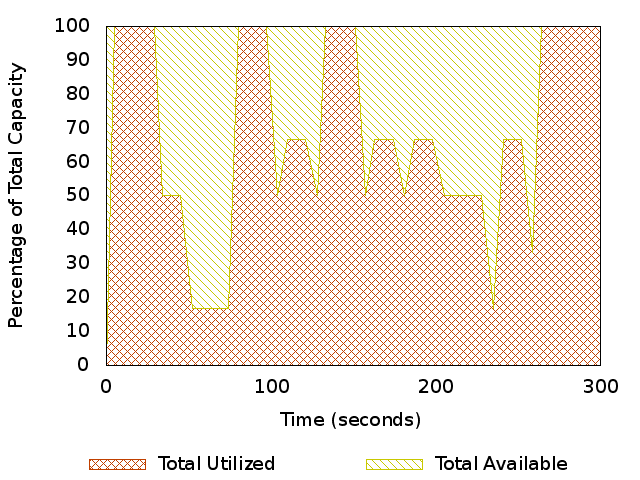
\includegraphics[width=0.65\textwidth,keepaspectratio]{graph_resource_util}
		\caption{Overall resource utilisation of the four ONs}
		\label{fig:resource-util-graphs}
\end{figure}


%%%%%%%%%%%%%%%%%%%%%%%%%%%%%%%%%%%%%%%%
\subsubsection{Credit Distribution}

Figure~\ref{fig:credit-distrib-graphs} shows the credit distribution among the four ONs during the 5 minutes of the experiment.
A node's credit is affected by how many VMs it shares and how much credit it spends to obtain VMs.
When a node shares most of its capacity, like ON f102 providing all its 3 VMs, 
it earns more credit and so maintains a high credit level during the experiment.
On the other hand, when a node continuously consumes VMs like ON f101 and f104, 
it keeps on spending any credit that it earns, so its credit does not increase beyond a certain level. 
Of particular interest is the behaviour of ON f103, which earns credit in the start and gets a spike in credit level halfway through the experiment, but then quickly spends it as it requests VMs from others.

Note that an ON's credit can be negative or higher than 100\% of the total credit 
because in the current implementation SN can allow requests from ONs with zero or or less than zero credit up to some extent. 
The ONs with zero or negative credit can, of course, continue to provide VMs and earn credit, they can only not request VMs if their credit is negative and below a certain threshold.
This allows the nodes without any credit an opportunity to continue participating in the system and increase their credit by contributing resources. 

%% FIGURE
\begin{figure}[tbp]
	\centering
		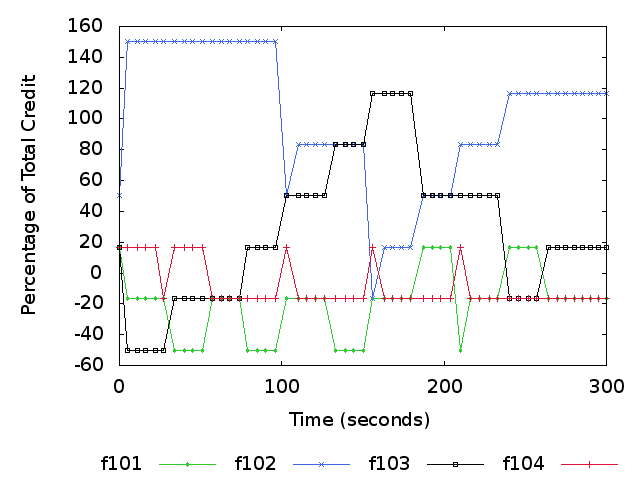
\includegraphics[width=0.65\textwidth,keepaspectratio]{graph_credit_distrib}
		\caption{Distribution of credit among the four ONs}
		\label{fig:credit-distrib-graphs}
\end{figure}


%%%%%%%%%%%%%%%%%%%%%%%%%%%%%%%%%%%%%%%%
\subsubsection{Success Ratio}

Figure~\ref{fig:success-ratio-graphs} shows the ratio of the fulfilled requests for each node, which is affected by the level of credit of the node and the amount of resources available in the system.
ON f104 has the most success since it requests only one VM at a time while ON f103 has the least success since it requests 3 VMs, which is half of the total shared VMs in the system. 
ON f101, on the other hand, gets its requests rejected because of the lack of credit. 
Therefore, this node has to wait to gain the needed credit.


%% FIGURE
\begin{figure}[tbp]
	\centering
	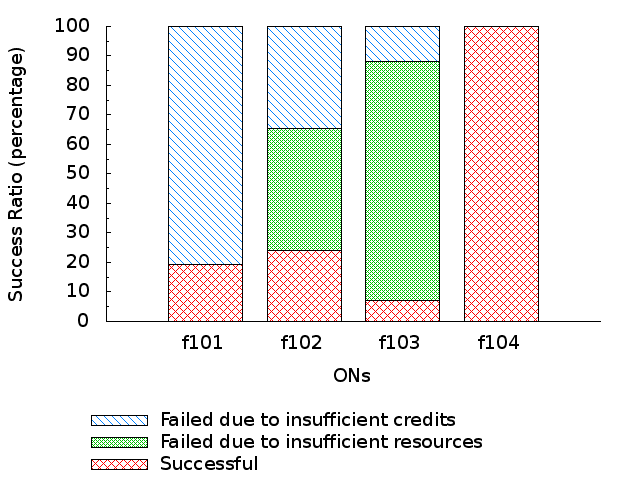
\includegraphics[width=0.65\textwidth,keepaspectratio]{graph_success_ratio}
	\caption{Ratio of fulfilled and rejected requests}
	\label{fig:success-ratio-graphs}
\end{figure}


%%%%%%%%%%%%%%%%%%%%%%%%%%%%%%%%%%%%%%%%
%%%%%%%%%%%%%%%%%%%%%%%%%%%%%%%%%%%%%%%%
\subsubsection{Resource Assignment in Federated Community Cloud Scenario}
\label{sec:resource-assign-federated}

In this experiment, we set up two local clouds, each with one SN and four ONs to study the federated community cloud scenario, as illustrated in Figure~\ref{fig:federated_cloud}.  
Table~\ref{tab:resource-distribution} shows the two cases with different number of VMs available in the two zones.
In the case of scarce capacity (case 1), the nodes in the SN1 zone share very few VMs compared to nodes in SN2 zone.
In the case of equal capacity (case 2), the nodes in both the zones share the same number of VMs.

%% TABLE
\begin{table}[tbp]
    \renewcommand{\arraystretch}{1.3}
   	\footnotesize    
    \caption{Two cases with different resource distribution between zones}
    \label{tab:resource-distribution}
    \centering

    \begin{tabular}{@{} l  c  c  c  c  c @{}}
    \hline
    \multicolumn{2}{c}{} 	& \multicolumn{2}{c}{Case 1: Scarce Capacity} & \multicolumn{2}{c}{Case 2: Equal Capacity}  \\ \hline
    SNs 					&       ONs     &   Total VMs   &   Shared VMs  &   Total VMs   &   Shared VMs \\ \hline
    \multirow{4}{*}{SN1}    &       ON1     &   3     	    &	1			&    3	        &	2   \\
                            &       ON2 	&	3	        &	1			&    3	        &	3   \\
                            &       ON3 	&	3	        &	1			&    3	        &	2   \\
                            &       ON4 	&	1	        &	1			&    1	        &	1   \\
    \hline
    \multirow{4}{*}{SN2}    &       ON1     &   3     	    &	2			&    3	        &	2   \\
                            &       ON2 	&	3	        &	3			&    3	        &	3   \\
                            &       ON3 	&	3	        &	2			&    3	        &	2   \\
                            &       ON4 	&	1	        &	1			&    1	        &	1   \\
    \hline
    \end{tabular}
\end{table}     

Figure~\ref{fig:multiple-snzone-graphs} shows the proportion of the requests fulfilled by VMs provided by the other zone.
With scarce capacity in SN1 zone, around 50\% of the requests are fulfilled by VMs provided by SN2 zone.
SN2 with sufficient capacity is able to meet most of the requests from VMs within the same zone, forwarding less than 15\% requests to the other zone.
In the second case, when both zones have the same available capacity, most of the requests get processed within the same zone for both the SNs.
This shows that a federated community cloud scenario extends the resources assigned to zones with limited capacity.

%% FIGURE
\begin{figure}[tbp]
	\centering
	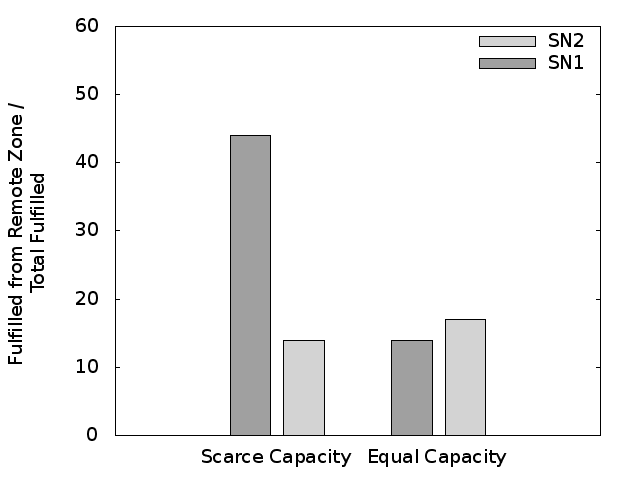
\includegraphics[width=0.55\textwidth,keepaspectratio]{graph_multiple_snzone}
	\caption{Resources assigned from different SN zones}
	\label{fig:multiple-snzone-graphs}
\end{figure}